\documentclass[a4paper,english]{report}
\usepackage[utf8]{inputenc}
\setcounter{secnumdepth}{3}
\usepackage{babel}
\usepackage{array}
%\usepackage{booktabs}
\usepackage{textcomp}
\usepackage{url}
\usepackage{multirow}
\usepackage{amsmath}
\usepackage{graphicx}
\usepackage[authoryear]{natbib}
\usepackage{nomencl}
\providecommand{\printnomenclature}{\printglossary}
\providecommand{\makenomenclature}{\makeglossary}
\makenomenclature
\usepackage[unicode=true,
 bookmarks=false,
 breaklinks=false,pdfborder={0 0 1},backref=section,colorlinks=false]
 {hyperref}
\usepackage{breakurl}
\usepackage{etoolbox}
\makeatletter
\patchcmd{\Ginclude@eps}{"#1"}{#1}{}{}
\makeatother

%\makeatletter
%\special{papersize=\the\paperwidth,\the\paperheight}

%\newcommand{\noun}[1]{\textsc{#1}}
%\providecommand{\tabularnewline}{\\}
%\newcommand{\lyxdot}{.}


\usepackage[colorinlistoftodos]{todonotes}
%\usepackage{placeins}
%\usepackage{parskip}



\usepackage{subcaption}
\usepackage{tikz}

\usepackage{array}

\usepackage{amssymb}


\usepackage{graphicx}

%\usepackage{booktabs}
%\newcommand{\otoprule}{\midrule[\heavyrulewidth]}

%\usepackage{pdflscape}
%\usepackage{bbding}
%\usepackage{pifont}

\makeatother

\begin{document}
\thispagestyle{empty}

\vspace*{3cm}

\begin{center}
{\LARGE{}Simplified Marine Cybernetics}
\par\end{center}{\LARGE \par}

\begin{center}
{\LARGE{}Laboratory Handbook }
\par\end{center}{\LARGE \par}

\begin{flushleft}
\vfill{}
\par\end{flushleft}

\begin{flushleft}

\includegraphics[scale=0.6]{fig/NTNU_logo.pdf}
\par\end{flushleft}

Faculty of Engineering Science and Technology\\
Department of Marine Technology

\clearpage{}\thispagestyle{empty}\vspace*{3cm}

\clearpage{}

\pagenumbering{roman}\setcounter{page}{1}

\vspace*{3cm}

\section*{Introduction}

This handbook is a simplified version of the Marine Cybernetics Laboratory Handbook, intended for use in TMR4243 - \textit{Marine Control Systems II}. The full Handbook can be found on Github(\url{https://github.com/NTNU-MCS/MC_Lab_Handbook}), with extensive information on all vessels and technical description of the different software.

\section*{Structure}
Chapter \ref{ch:marine_cybernetics_laboratory_equipment} describes the different equipment found in the Laboratory, and how to use it. 

Chapter...

\newpage{}
\tableofcontents{}
\clearpage
\pagenumbering{arabic}
\chapter{Marine Cybernetics Laboratory equipment}\label{ch:marine_cybernetics_laboratory_equipment}
\section{Introduction}
The laboratory is equipped for experimental testing of marine control systems and hydrodynamic tests. It consists of a wave basin with an advanced instrumentation package and a towing carriage. The basin, depicted in Figure \ref{fig: Marine cybernetics laboratory basin-1}, has dimensions 40m x 6.45m x 1.5m (LxBxD). The laboratory consists of the following fixed equipment: 
\begin{itemize}
	\item Qualisys Motion Capture System
	\item Towing Carriage
	\item Wave Generator
	\item Video-camera
\end{itemize}
These parts are thouroghly described in the next sections, with a user manual and technical description of the equipment. 

\begin{figure}[h!]
	\centering 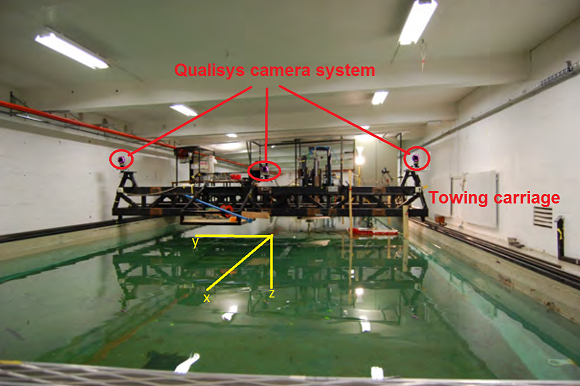
\includegraphics[width=0.95\textwidth]{fig/mc_lab} 
	\caption{Marine cybernetics laboratory basin}
	\label{fig: Marine cybernetics laboratory basin-1}
\end{figure}

\subsection{Safety}\
\subsubsection{Personnel injury}
\paragraph{Drowning}
It is required to have two or more persons present when using the basin.
\paragraph{Electric shock}
The towing catenary should not be approached or touched.
\paragraph{Carriage collision}
It is forbidden to run the towing carriage when there are people alongside the basin.
\paragraph{Thruster blade cuts}
Vessels must stay in the water as long as actuators are active. Before removing the vessels from the water, the control system must be stopped and disabled, for instance by undeploying in the VeriStand project.

\subsubsection{Material damage}
\paragraph{Cybership Enterprise 1}
\begin{description}
	\item [{Water~damage:}] CSE1 is not waterproof and has excessive thrust capability which can inflict large roll angles. The risk of water on deck is reduced through thrust limitation and HIL testing before application of new control algorithms. 
	\item [{Propeller~dry~running:}] BT must only be run in water. Before removing the vessel from the water, the control system must be stopped and the VeriStand project undeployed.
	\item [{Loss~of~laptop~control:}] Wireless network instability may result in loss of connection between the laptop user interface and the cRIO. In this event, fall back to manual thruster control, by pushing 
\includegraphics[scale=0.4]{fig/sixaxis_triangle} on the Sixaxis.
	\item [{Loss~of~position~measurement:}] -
	\item [{Total~loss~of~control:}] Pull the vessel with a boat hook. Keep the CSE1 in water while disconnecting batteries.
\end{description}

\paragraph{Towing carriage}
Stop before automatic stop at high speeds.

\clearpage{}

\section{Qualisys Motion Capture System}
Qualisys provides 6 degrees of freedom data tracking. The system has millimeter precision, works in real time and is configured to 50Hz.

The positioning system consists of three Oqus high speed infrared cameras registering infrared reflectors placed on the vessel. Peer-to-peer (P2P) networking is used to transmit camera data to a dedicated computer running Qualisys Track Manager (QTM) software. QTM performs triangulation and broadcasts the vessel position over the wireless network. The system is operated from a dedicated PC in the Lab, labeled with \textit{QTM surface vehicle}. \todo{Add info on zyx-convention}

\subsection{User Manual}
\subsubsection*{Start Qualisys Track Manager}
\begin{enumerate}
	\item Execute the program. The first displayed window is as in Figure \ref{fig: Qualisys Track Manager start window}.
		\begin{figure}[!h]
			\centering 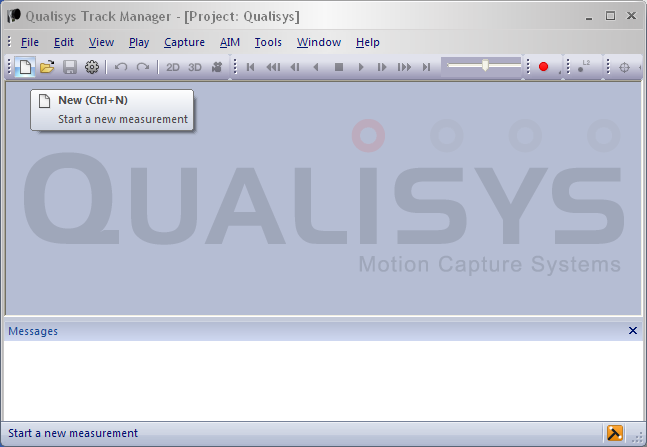
\includegraphics[width=1\textwidth]{fig/qualisys_new} 
			\caption{Qualisys Track Manager start window}
			\label{fig: Qualisys Track Manager start window}
		\end{figure}
	\item Push the white sheet icon to start a new measurement. The main window should then display the 2D view, as in Figure \ref{fig: Qualisys Track Manager 2D view}.
		\begin{figure}[!h]
			\centering 
			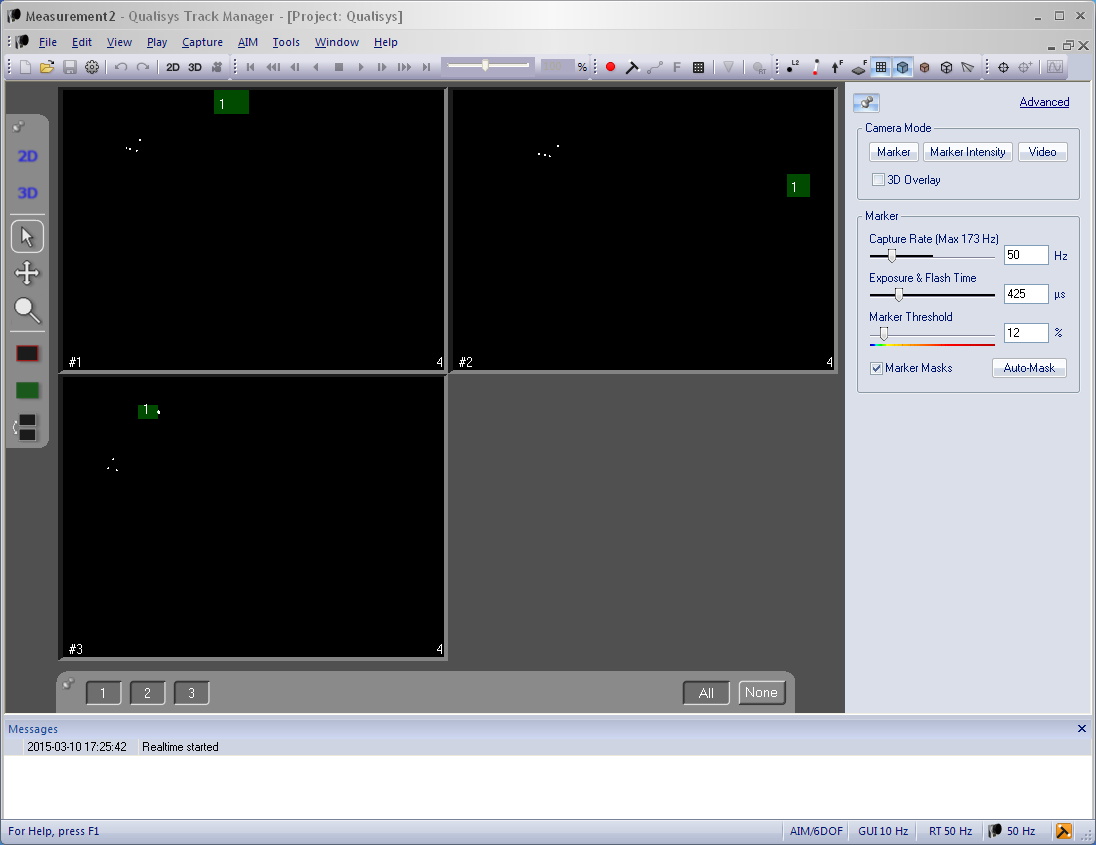
\includegraphics[width=1\textwidth]{fig/qualisys_3cams} 
			\caption{Qualisys Track Manager 2D view} 
			\label{fig: Qualisys Track Manager 2D view}
		\end{figure}
	The squares numbered \#1, \#2 and \#3 show the basin as seen from the respective cameras. The white dots are the vessel reflectors. A minimum of three reflectors must be visible in each camera. 
\end{enumerate}

\subsubsection*{Aquire body}
\begin{enumerate}
	\item Push the gear icon to access Project Options. Navigate to 6DOF Tracking,
	as in Figure \ref{fig:Qualisys-Track-Manager6DOF}.
	\begin{figure}[!h]
		\centering 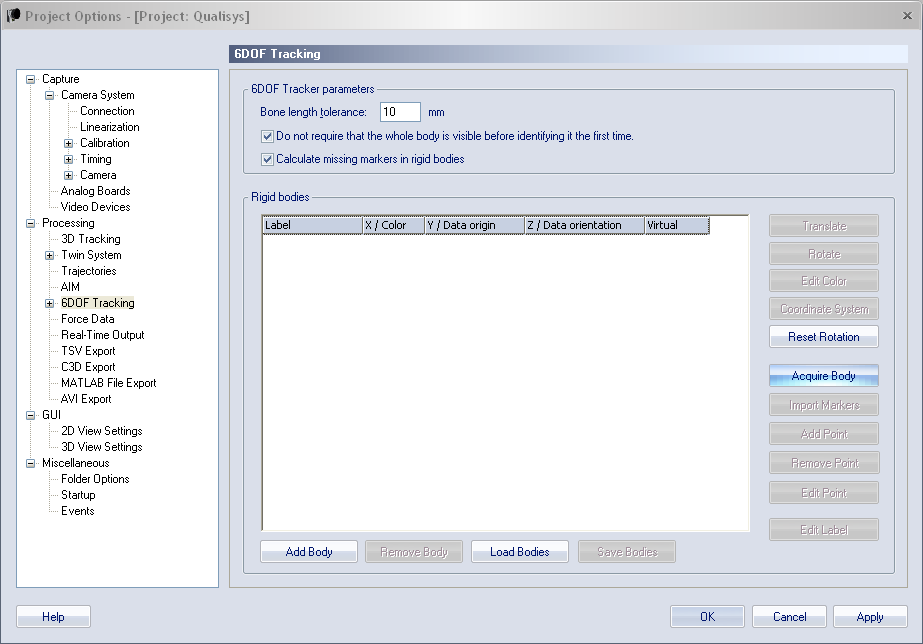
\includegraphics[width=1\textwidth]{fig/qualisys_6dof} \caption{\label{fig:Qualisys-Track-Manager6DOF}Qualisys Track Manager 6 DOF
			Tracking}
	\end{figure}
	\item Remove previous bodies, if any.
	\item Align the vessel with desired heading 0 and push ``Acquire Body''
	to get the position of the reflectors. A list appears, as in Figure
	\ref{fig:Qualisys-Track-ManagerAquiredBody}. 
	\begin{figure}[!h]
		\centering 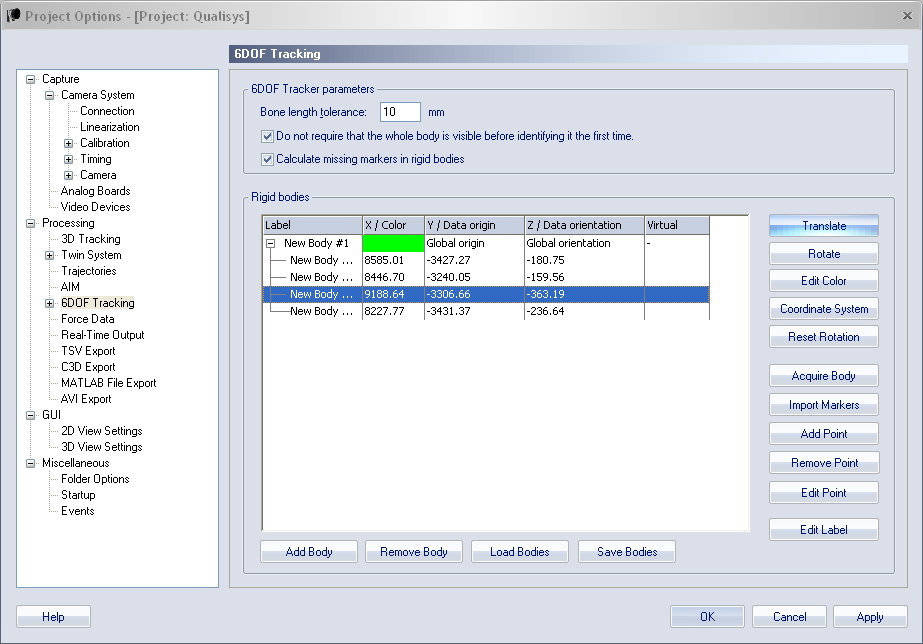
\includegraphics[width=1\textwidth]{fig/qualisys_orientating}
		\caption{\label{fig:Qualisys-Track-ManagerAquiredBody}Qualisys Track Manager
			aquired body}
	\end{figure}
	\item To redefine the body fixed coordinate frame 
	
	\begin{enumerate}
		\item Chose a reference reflector. As highlighted in Figure \ref{fig:Qualisys-Track-ManagerAquiredBody}, it may be practical to choose the highest-most, in this case reflector 3.
		\item Push ``Translate'' and enter the coordinates of the chosen reflector in the desired frame. In Figure \ref{fig:Qualisys-Track-Managertranslate}, reflector 3 is set at $x,y,z=\left(0.550,0,-0.500\right)$. 
		\begin{figure}[!h]
			\centering 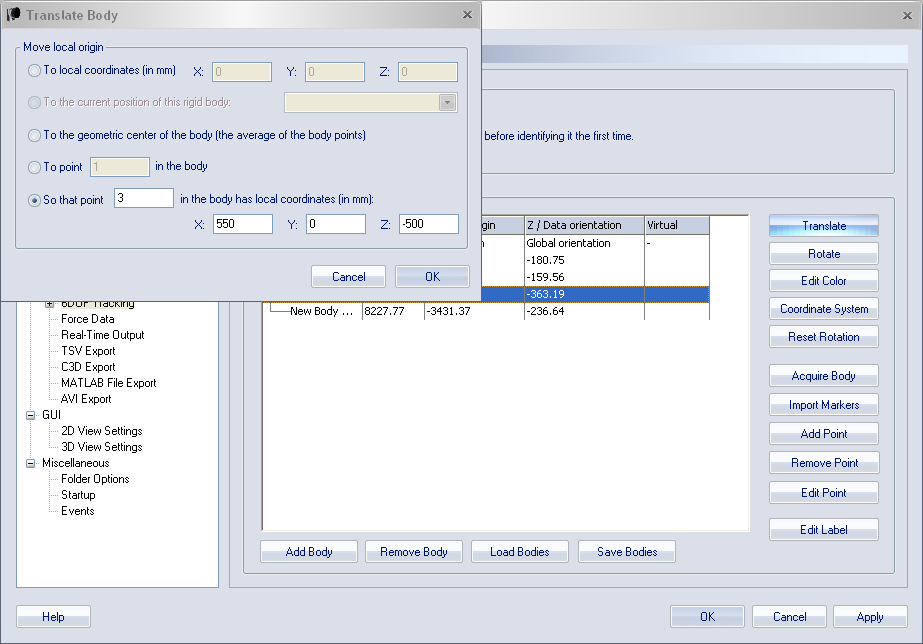
\includegraphics[width=1\textwidth]{fig/qualisys_orientating2}
			\caption{\label{fig:Qualisys-Track-Managertranslate}Qualisys Track Manager
				translate body}
		\end{figure}
		Figure \ref{fig:Qualisys-Track-Managertranslated} shows the resulting coordinates after translation.
		\begin{figure}[!h]
			\centering 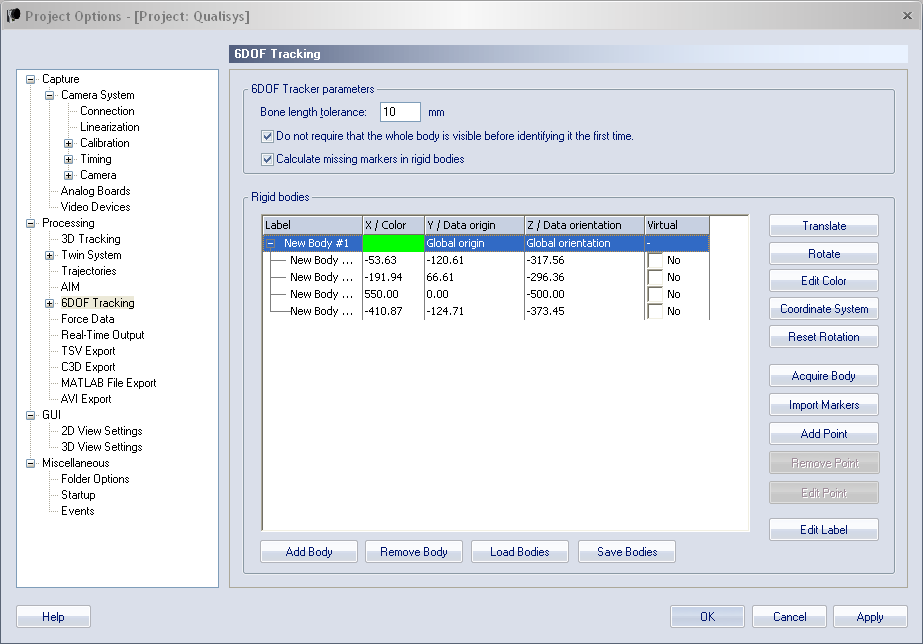
\includegraphics[width=1\textwidth]{fig/qualisys_orientating3}
			\caption{\label{fig:Qualisys-Track-Managertranslated}Qualisys Track Manager translated body}
		\end{figure}
	\end{enumerate}
	\item Finally, select 3D view to confirm that the body-fixed frame is indeed located as desired, as in Figure \ref{fig:Qualisys-Track-Managerr3D}.
	\begin{figure}[!h]
		\centering 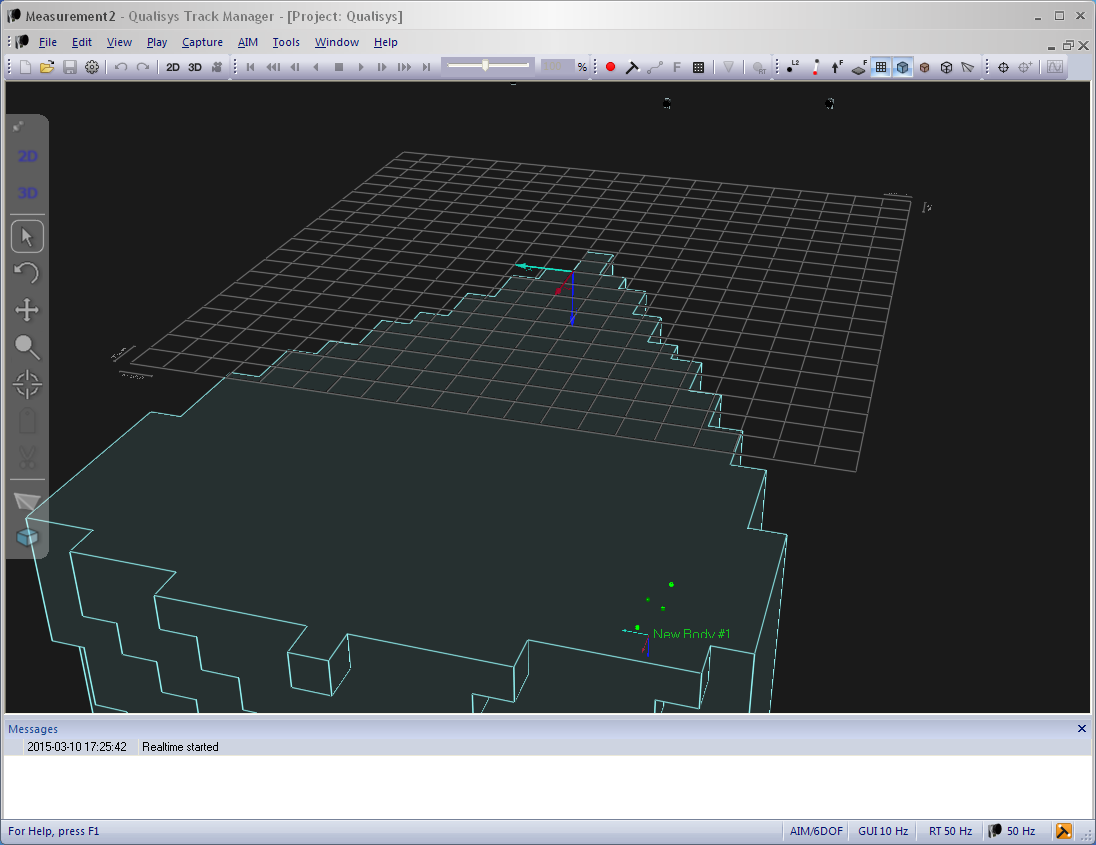
\includegraphics[width=1\textwidth]{fig/qualisys_3d} \caption{\label{fig:Qualisys-Track-Managerr3D}Qualisys Track Manager 3D view}
	\end{figure}
\end{enumerate}

\subsubsection*{Troubleshooting}
\paragraph*{Long waiting for camera}
\begin{figure}[!h]
	\centering 
	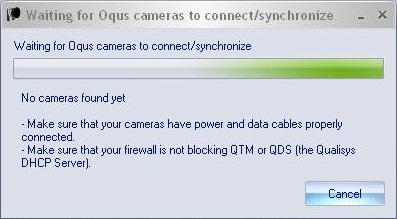
\includegraphics[scale=0.45]{fig/qualisys_waiting_to_connect}
	\caption{Qualisys Track Manager waiting for cameras}
	\label{fig:Qualisys-Track-ManagerWaiting}
\end{figure}
If the operation depicted in Figure \ref{fig:Qualisys-Track-ManagerWaiting} is unsuccessful after a couple of minutes, reboot the cameras by unplugging and reconnecting the power cord on the rack.
\clearpage{}
\subsection{Importing Data from the Qualisys System into ROD and MATLAB(Linux)}
The following approach may be used to read Qualisys data into ROS and MATLAB. The method is convenient for Qualisys data into to MATLAB independent on whether the rest of the system use ROS or not. The method, as described is limited to Linux-operating systems.

The first part of the manual describe how import Qualisys data into ROS, while the second part describe how to get the data from ROS into MATLAB/Simulink.

Please note the following: 
\begin{itemize}
	\item In the manual, the dollar sign \$ indicate a line of text that should be written in the Linux- terminal window.
	\item In the manual gedit is used as text editor. This can be replaced with the readers favourite text editor.
	\item The manual is written and tested for ROS-Indigo and MATLAB 2015b. It is based on MATLAB's manual for importing custom messages \citep{MathWorks2016}, which is and adapted and expanded to fit that of the MC lab and the Qualisys system.
	\item You need MATLAB version 2015a or newer in order to proceed with the MATLAB section of the manual.
\end{itemize}

\subsubsection{Manual}
If not already installed on the machine you should start by installing ROS. Follow the instructions on the ROS download page: \url{http://wiki.ros.org/indigo/Installation/Ubuntu}.

You should now make a ROS workspace in your home directory:

\begin{verbatim}$mkdir -p ~/catkin_ws/src 
$cd ~/catkin_ws/src
$catkin_init_workspace\end{verbatim}

You now need to make sure that one are sourcing the setup.bash file in your ROS workspace each time you open your terminal window. This can be done by changing the bash file with the following command:

\begin{verbatim}$ echo "source ~/catkin_ws/devel/setup.bash" >> ~/.bashrc\end{verbatim}

Now import the Qualisys driver from GitHub. (The driver \citep{KumarRobotics2016} is avaiable through the Apache License )

\begin{verbatim}$ cd ~/catkin_ws/src
$ git clone https://github.com/KumarRobotics/qualisys
$ cd ~/catkin_ws
$ catkin_make\end{verbatim}

Open the qualisys.launch file in a text-editor

\begin{verbatim}$ sudo gedit ~/catkin_ws/src/qualisys/launch/qualisys.launch\end{verbatim}

Edit the ip address and port number for the Qualisys system. (As of March 2016 the IP is: 192.168.0.10 and the port is 22222 )

The driver should now be set for interfacing with Qualisys in ROS. To test it, first check that you are able to ping the Qualisys system over the MC lab WiFi.

\begin{verbatim}$ ping 192.168.0.10\end{verbatim}

If you successfully pinged the qualisys system it should now be possible to listen to the data from the Qualisys system.

(Note that the Qualisys system need to recognize the IR-markers in the MC lab in order to transmit data. It may be smart to first to check that the computer running Qualisys software in the MC-Lab sees the marker)

\begin{verbatim}$ roslaunch qualisys qualisys.launch
$ rostopic list\end{verbatim}

The command ``rostopic list'' prints the ROS active ROS topics. It should now be printed a qualisys topic in terminal. The name will depend on the name set on the Qualisys computer. In this manual the topic is named /qualisys/CSE1.

You can now listen to the data as it is published to ROS

\begin{verbatim}$ rostopic echo /qualisys/CSE1\end{verbatim}

\subsubsection{Getting Qualisys data to MATLAB}

The message sent from the Qualisys system is a custom message that MATLAB does not recognize (most messages in ROS is not custom, and will be recognized by MATLAB). In order to get the Qualisys data into MATLAB you one to facilitate so that MATLAB recognize the custom message.

Start by creating a new folder \textasciitilde{}/qualisysDir. Now copy the folder named qualisys, located in \textasciitilde{}/catkin\_ws/src and paste it into the folder \textasciitilde{}/qualisysDir

Now one want to edit the package file so that MATLAB recognizes the messages.

\begin{verbatim}Sudo gedit ~/qualisysDir/qualisys/package.xml\end{verbatim}

Add the following two lines somewhere in the main body of the package.xml file.

\begin{verbatim}<build_depend>geometry_msgs</build_depend>
<build_depend>std_msgs</build_depend>\end{verbatim}

Now open MATLAB. The first step in MATLAB is to download the ROS custom message package. Type the following lines into the MATLAB command window, and follow instructions to download the ROS custom message package.

\begin{verbatim}roboticsAddons (in MATLAB 2016)
roboticsSupportPackages  (in MATLAB 2015)\end{verbatim}

When the download is finished paste the following commands in the MATLAB command window.

\begin{verbatim}folderpath= '~/qualisysDir'
rosgenmsg(folderpath)\end{verbatim}

Now follow the instructions generated by MATLAB in order generate the needed message type. In this process you may need allow writing permission to the file ``pathdef.m''

You are now ready to get the data into MATLAB.

Remember that the Qualisys node always need to be launched before reading signals in MATLAB.

\begin{verbatim}roslaunch qualisys qualisys.launch\end{verbatim}

You can now get the data into Simulink by the Subscriber block, or to MATLAB workspace by typing the following commands:

\begin{verbatim}Subb = rossubscriber('/qualisys/CSE1');
posedata = receive(Subb,10);\end{verbatim}

\clearpage

\section{Towing carriage}
\begin{figure}[htb!]
	\centering 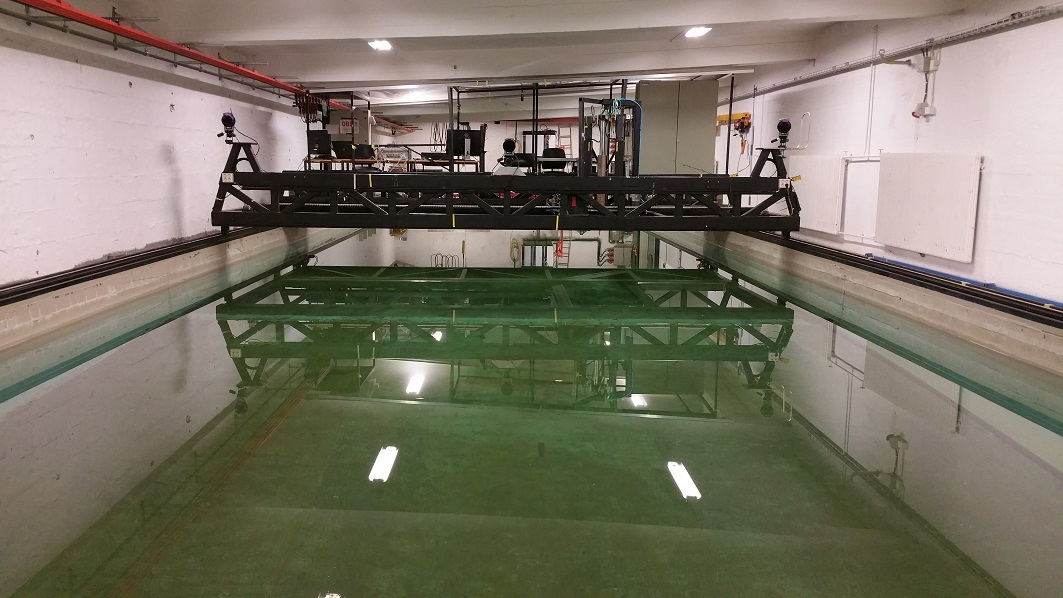
\includegraphics[width=1\textwidth]{fig/towing_carriage}
	\caption{Towing carriage}
	\label{fig: Towing carriage}
\end{figure}
The scope of this section is to explain how to safely operate the carriage without any damage towards humans or equipment. 

\subsection{Preparation before startup}
To start with, you must make sure that any items mounted or fixed to the carriage are securely fitted, so they don't prevent the operation of the carriage. All personnel must stay on the operation platform during the travel of any axis.

Locate the Emergency Button and place it so that you can easily reach it from where you are sited. DO NOT USE THE EMERGENCY BUTTOM AS A BRAKE. YOU MUST ONLY OPERATE IT WHEN YOU ARE IN REAL EMERGENCY SITUATIONS.

\subsubsection*{Operation console}
\begin{figure}[htb!]
	\centering 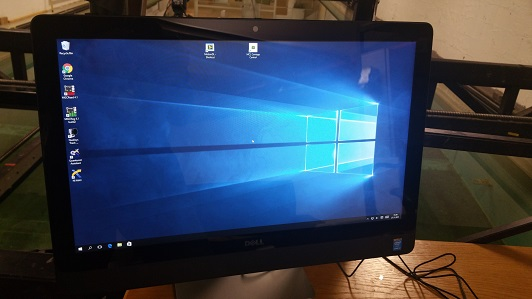
\includegraphics[width=0.8\textwidth]{fig/towing_console}
	\caption{Towing console}
	\label{fig: Towing console}
\end{figure}

The operation console is an All-in-one PC. The Power button is on the bottom right side of the screen. If the operation panel is not on the desktop, you can start it by double clicking on desktop Icon, shown in Figure \ref{fig: Towing console}.

\subsection{Manual Operation of the Carriage}
\subsubsection*{Setup}
\begin{figure}[htb!]
	\centering 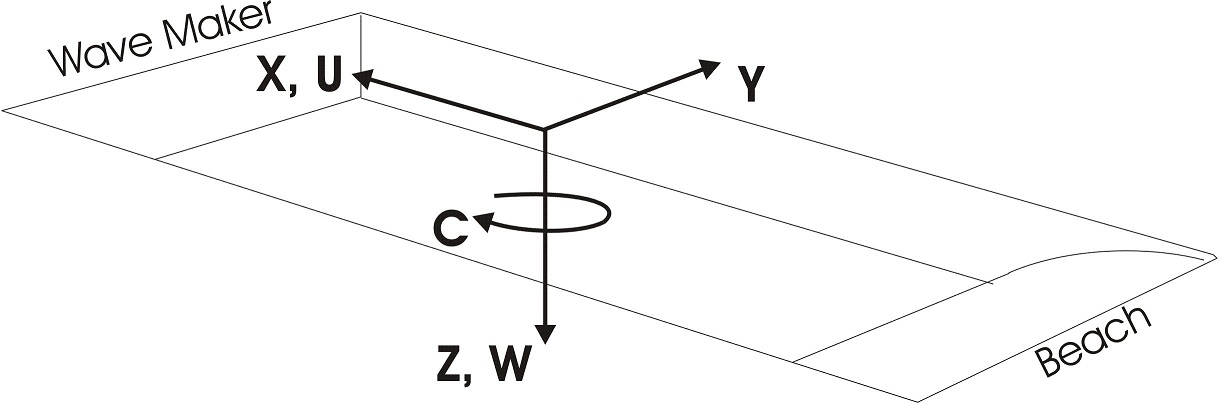
\includegraphics[width=0.8\textwidth]{fig/towing_coordinate_sketch}
	\caption{Coordinate system}
	\label{fig: Towing carriage-1}
\end{figure}

\begin{figure}[htb!]
	\centering 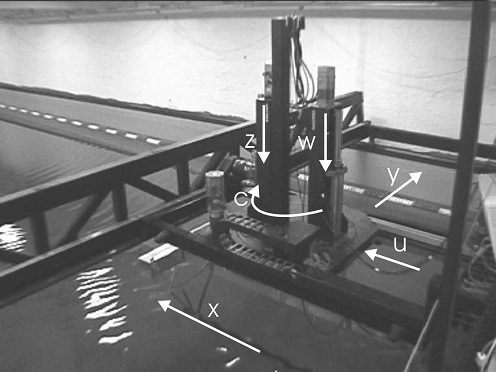
\includegraphics[width=0.8\textwidth]{fig/towing_coordinate_photo}
	\caption{Coordinate system}
\end{figure}

\begin{table}
	\centering{}%
	\begin{tabular}{lllllll}
		\hline 
		& \multicolumn{2}{l}{Forward/Backward} & \multicolumn{2}{l}{Acceleration} & \multicolumn{2}{l}{Position}\tabularnewline
		Axis & \multicolumn{2}{l}{Speed} & \multicolumn{2}{l}{Deceleration} & \multicolumn{2}{l}{Pos./Neg. Limit}\tabularnewline
		\hline 
		X & 0 - 2.0 & {[}m/s{]}  & \% of 0 - 0.5 & $\text{m/\ensuremath{s^{2}}}$ & 0 - 22 & {[}m{]}\tabularnewline
		Y & 0 - 1.0 & {[}m/s{]}  & \% of 0 - 1.0 & $\text{m/\ensuremath{s^{2}}}$ & 0 - 4.5 & {[}m{]}\tabularnewline
		U & 0 - 1.0 & {[}m/s{]}  & \% of 0 - 1.0 & $\text{m/\ensuremath{s^{2}}}$ & 0 - 1 & {[}m{]}\tabularnewline
		C & 0 - 10  & {[}deg/s{]} & \% of 0 - 20 & $\text{deg/\ensuremath{s^{2}}}$ & 0 - 255 & {[}deg{]}\tabularnewline
		Z & 0 - 1.0 & {[}m/s{]}  & \% of 0 - 2.0 & $\text{m/\ensuremath{s^{2}}}$ & 0 - 0.5 & {[}m{]}\tabularnewline
		W & 0 - 1.0 & {[}m/s{]}  & \% of 0 - 2.0 & $\text{m/\ensuremath{s^{2}}}$ & 0 - 0.5 & {[}m{]}\tabularnewline
		\hline 
	\end{tabular}\caption{\label{tab: Operation Limit}Operation Limit}
\end{table}

\begin{figure}[htb!]
	\centering 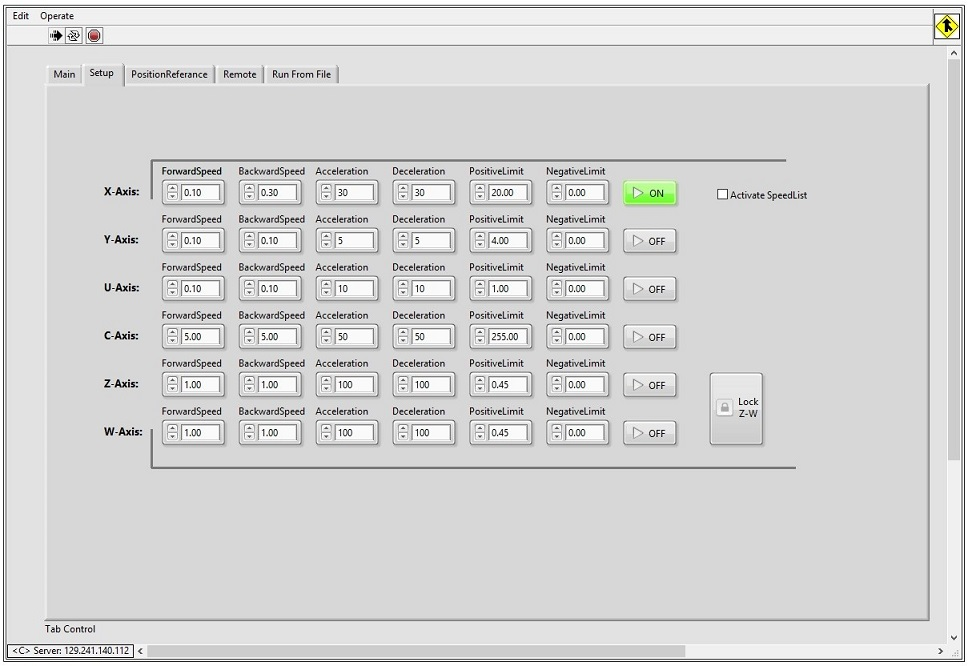
\includegraphics[width=0.8\textwidth]{fig/towing_parameteres}
	\caption{Setup}
	\label{fig: Towing parameters}
\end{figure}

It is very important to select the Setup tab first before you start any operation of the carriage. As you can see in Figure \ref{fig: Towing parameters}, it is possible to change the travel parameters for all available axes. In principle, all axis parameters have different range limits. These are listed in Table \ref{tab: Operation Limit}.

All axes can be activated or deactivate by using the ON button.

For the X axis it is possible to activate a list of predefined Forward speeds. You will then have the ability to automatically change to a different speed on the next run. The list can be edited in the Main Tab Window.

By selecting the ``Lock Z-W'' button the Z-W axis will operate in parallel. They will use the Z-axis parameter setup.

\subsubsection*{Main/Standard Operation}
\begin{figure}[htb!]
	\centering 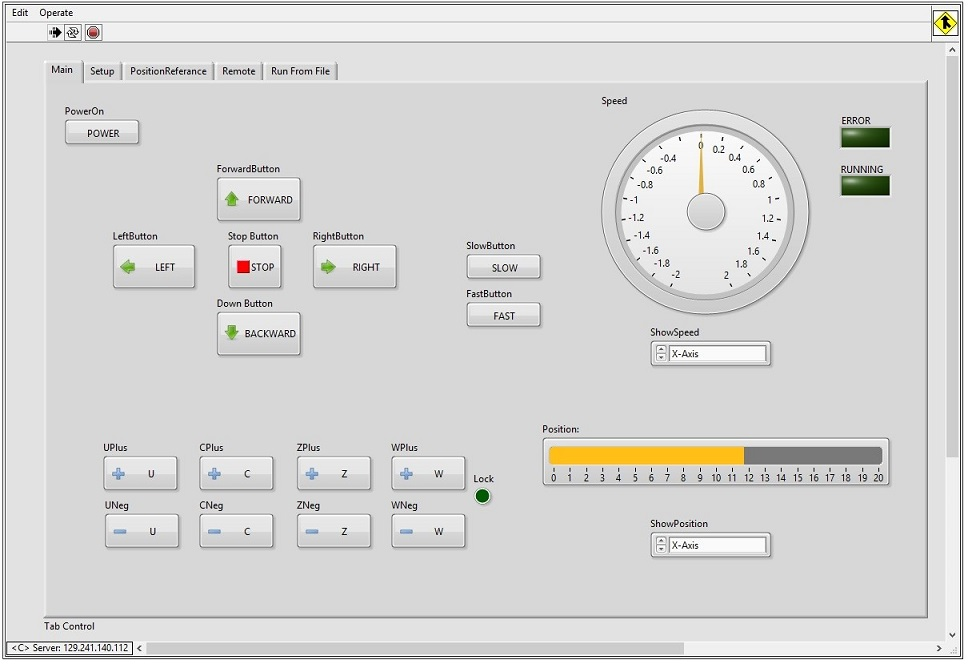
\includegraphics[width=0.8\textwidth]{fig/towing_main} 
	\caption{Main}
	\label{fig: Towing main}
\end{figure}

All the activated axes will operate within the limits set in the Setup. Only one axis can operate at a time. If you hit the button for another axis than the running one, it will instantly stop and new one will start running. To stop the running axis, simply hit the stop button. If no buttons are operated carriage axis will run it hit limit position of the current axis.

If an error occurs, for some reason, it can be cleared by hitting the ``Power'' button. If the error keeps reoccurring, please look at the Troubleshooting section of this document or contact responsible MC Lab personnel.

The current speed and position of the active axis are displayed referred to the selected limits.

\subsection{Operation Controlled automatically from PC}

\begin{figure}[htb!]
	\centering 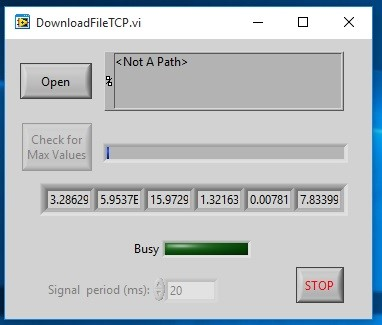
\includegraphics[width=0.8\textwidth]{fig/towing_runfromfile}
	\caption{Run From File}
	\label{fig: Towing main-1}
\end{figure}


\subsubsection*{The Trajectory Input File}

All trajectories must be defined in a .mcl input file. The format of the file is slightly more general than allowed here and is the same as for the sloshing rig input. The entries in the file are
\begin{enumerate}
	\item Time Step in ms, double precision integer (int32). Must be set to 10.
	\item Number of channels, double precision integer (int32). Must be 6.
	\item Position references in sequence: X(1),Y(1),U(1),C(1),Z(1),W(1), X(2),Y(2), double precision real (float32).
\end{enumerate}
The following MTALAB lines write the matrix body (6xN) to file on
the correct format:
\begin{verbatim}
fid=fopen(filename,'wb');
head=[10;6];
count=fwrite(fid,head,'int32');
count=count+fwrite(fid,body,'float32');
fclose(fid); 
\end{verbatim}

The resulting input file must be transferred to the realtime computer at /home/ntuser/inputpos.mcl. Normally this is done automatically when the Load button on the LabVIEW GUI is pressed. 

\begin{figure}[htb!]
	\centering 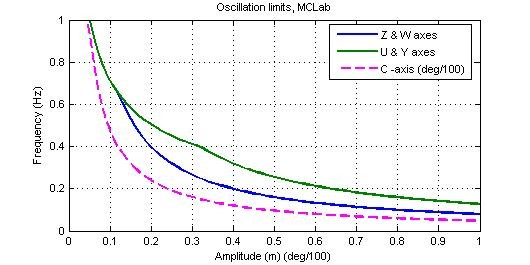
\includegraphics[width=0.8\textwidth]{fig/towing_ampvsfreq}
	\caption{\label{fig: Towing main-1-1}Operation Limit Amplitude vs. Frequency}
\end{figure}
\subsection{Troubleshooting}
\subsection{Note}
When the wagon is moving, no one is allowed to move on the sides of the basin.
\clearpage{}

\section{Wave Generator}\label{sec:wave_generator}
The wave maker is a single paddle wave making machine with a width of 6 meter and it is equipped with an Active Wave Absorption Control System (AWACS 2). The single paddle wave generator is controlled by a dedicated computer. The machine can produce both regular and irregular waves because of the DHI Wave Synthesizer the system has. Available spectrum are first order Stoke, JONSWAP, Pierson-Moskowitz, Bretschneider, ISSC and ITTC. Table \ref{tab:Wave generator capacity-1} summarizes the generation capacity.
\begin{table}[h!]
	\centering{}
	\begin{tabular}{lll}
		\hline 
		& Height {[}m{]} & Period T {[}s{]}\tabularnewline
		\hline 
		Regular waves & $H<0.25$ & 0.3 - 3.0\tabularnewline
		Irregular waves & \textbf{$H_{s}<0.15$} & 0.6 - 1.5\tabularnewline
		\hline 
	\end{tabular}\caption{\label{tab:Wave generator capacity-1}Wave generator capacity}
\end{table}
\subsection{User Manual}
\todo{Add a description on how to use the system once the NEW wave generator is installed(fall 2017)}
\clearpage{}
\section{Video-Camera System}
The laboratory is equipped with 2 high-resolution cameras for recording of activity in the basin, one on each side. The cameras are remotely operated from a dedicated PC in the command center using the \textit{Intelligent Video Management System 4200 (iVMS-4200 client)} software. The computer is located on the floor, is connected to the TV-monitor mounted on the wall, and has wireless mouse and keyboard(labeled \textit{Camera system}). The software user-interface is illustrated in Figure \ref{fig:userinterface_iVMS-4200}. 

The manual control of the cameras are found in the \textit{PTZ Control} tab. The cameras feature auto-tracking of objects, which is enabled by right-clicking in the video window. The menu is illustrated in Figure \ref{fig:userinterface_iVMS-4200}, with highlighted options for auto-tracking and manual control of the camera position. 
The camera system also support recording. Note that the recorded files are large, typically several GB for some minutes of recorded video. Hence, the files should be \textit{moved} to a USB-disk(and not copied). The recorded files are found in the path: \path{C:\ivms4200\video\RecordFile\YYYYMMDD}.
\begin{figure}[htb!]
	\centerline{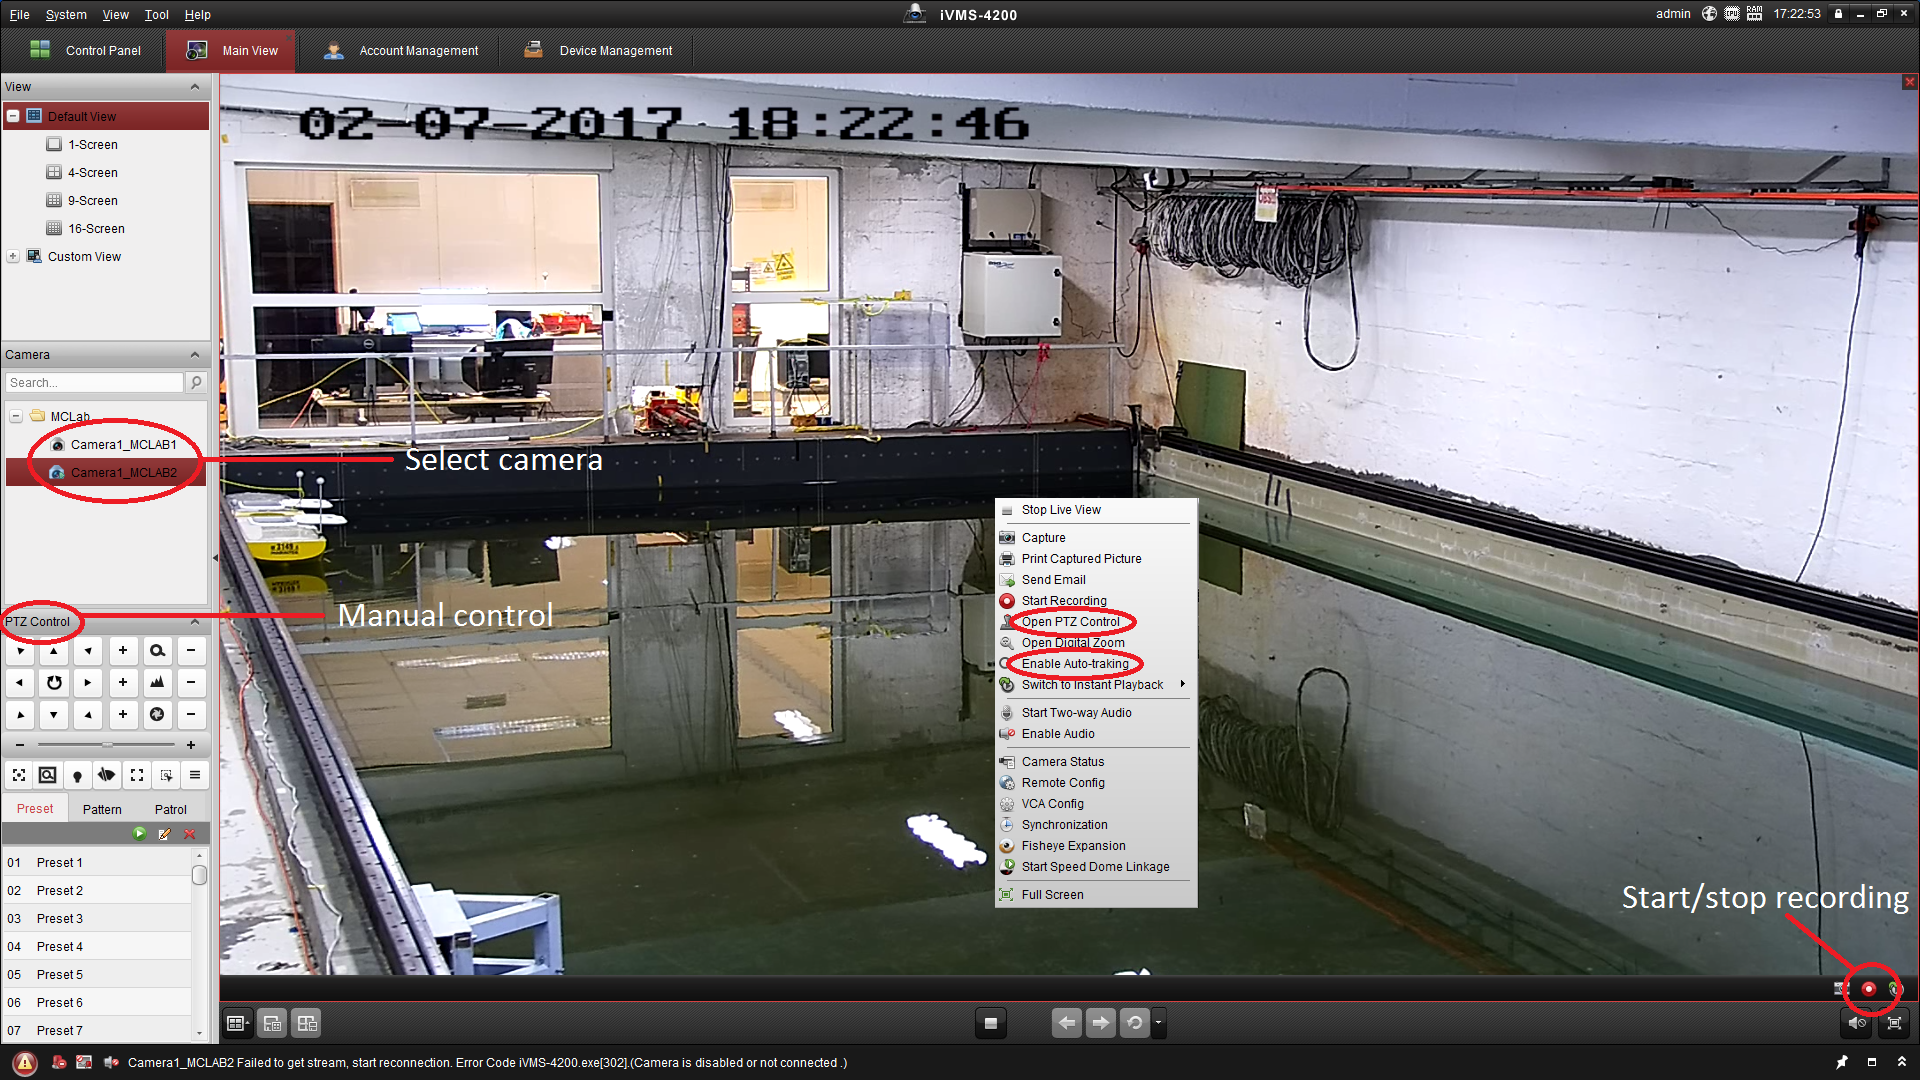
\includegraphics[width=1.4\linewidth]{fig/Camera_userinterface.png}}
	\caption{User interface iVMS-4200 camera system}
	\label{fig:userinterface_iVMS-4200}
\end{figure}

\clearpage
\bibliographystyle{elsarticle-harv}
\bibliography{referencesl}
\end{document}